% !TEX root = ../lifeonbrane3.tex
%





%\subsection{`Bubbles' on the brane}\label{bubblesX}


In this appendix, we consider a simple but surprising class of RT surfaces. In particular, we show below that there are closed extremal surfaces with the topology of a sphere, \ie $S^{d-1}$ in the locally AdS$_{d+1}$ bulk geometry. In empty AdS space, one could consider such spherical surfaces, but their area would be extremized when they collapse to zero size. In the present case, we will show that in certain situations, the spherical RT surfaces can be supported at finite size by the brane.  To illustrate the situation, we continue with the special case of $d=3$ as in section \ref{sec:examples}, and afterwards comment on the situation with general $d$. 
%
%\begin{figure}[h]
%\begin{center}
%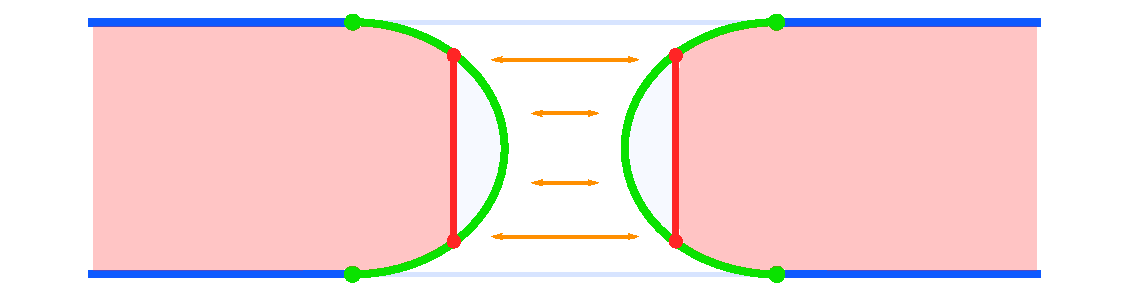
\includegraphics[scale=0.2]{images/bubble}
%\caption{One half of an RT bubble supported on the brane. \rcm{Lets illustrate this in the `style' of figure \ref{fig:EWs}.}}
%\label{figbubble}
%\end{center}
%\end{figure}

\begin{figure}[h]
	\def\svgwidth{0.8\linewidth}
	\centering{
		\input{bubble.pdf_tex}
		\caption{An RT `bubble' on the brane: even for the vacuum, when $\Gbr<0$ the competing bulk and brane area terms can lead to a stable extremal surface, which is  homologous to the entire time slice for the boundary CFT. The entanglement wedge then corresponds to the shaded red region. Since the two sides of the brane are glued together, the RT surface has the topology of $S^{d-1}$. }
		\label{figbubble}
	}
\end{figure}

Consider the geometry illustrated in figure \ref{figbubble}. On either side of the brane, we have a disk satisfying $\zeta=$constant, \ie satisfying eq.~\reef{zetap} with $P_0=0$. Hence locally these surfaces extremize the entropy functional \reef{area} in the bulk. However, rather than extending out to the asymptotic boundary, as shown in the figure, the two disks intersect the brane and meet at some radius $\pb$.  Hence this RT surface has the topology of a sphere and we use the nomenclature `bubble' to describe these surfaces. For $d=3$, the generalised entropy \reef{eq:sad} of this bubble is
\begin{align}\label{Agenbubble}
\sgen&=\frac{\pi L^2}{\Gbk} \left(  \sqrt{1+\pb^2}-1  + \lamb\, \pb \right) +2\,\lgb 
\end{align}
with $\lamb$ defined in eq.~\eqref{newdefs}. We have also included the topological term introduced in eq.~\reef{Euler3}.
Of course, since these surfaces never reach the asymptotic boundary, this quantity is finite, \ie there are no UV divergences in eq.~\reef{Agenbubble}. 

Extremizing eq.~\reef{Agenbubble} with respect to the radius of the bubble, we find
\beq\label{gamdot}
\partial_{\pb}\sgen=0 \qquad
\implies\qquad \frac{\pb}{\sqrt{1+\pb^2}}=-\lamb=-\frac{\Gbk}{2L\,\Gbr}\,.
\eeq
Now recall that we will always have $\Gbk>0$, but considered the possibility of $\Gbr$ becoming negative in section \ref{sec:examples}. Let us first consider the case $\lamb\ge 0$, which implies $1/\Gbr\ge 0$. In this case, we can not satisfy eq.~\reef{gamdot}, since both the bulk and brane contributions to the generalised entropy \eqref{Agenbubble} are positive and monotonically increasing functions of $\pb$. Therefore the minimum lies at $\pb=0$, \ie where the bubble collapses to zero size -- see figure \reef{figAbubble}. 

Of course, the more interesting scenario is when $\lamb$, and hence
$1/\Gbr$, are negative. Then eq.~\reef{gamdot} has the solution
\begin{align}
\pbo=-\frac{\lamb}{\sqrt{1-\lamb^2}}\,,
\label{cookie}
\end{align}
for which the generalized entropy \reef{Agenbubble} becomes
\begin{align}\label{Sbubble}
\sgen= \frac{\pi L^2}{\Gbk} \left( \sqrt{1-\lamb^2} - 1 \right)+2\,\lgb .
\end{align}
We note that these expressions are only sensible for $-1<\lamb<0$. In fact, for $\lamb<-1$, there is no minimum for the generalized entropy \reef{Agenbubble}, \ie there is no solution for eq.~\reef{gamdot}, and rather $\pb$ runs off to infinity -- see figure \reef{figAbubble}.  This is, perhaps, not so surprising since we can see from eq.~\reef{Newton34} that this regime is pathological, with the graviton localized on the brane becoming a ghost.

Therefore we only consider the regime $-1<\lamb<0$ where eqs.~\reef{cookie} and \reef{Sbubble} apply. As illustrated in figure \reef{figAbubble}, eq.~\reef{cookie} is indeed the global minimum of the generalized entropy \eqref{Agenbubble}. We might note that the sum of the bulk and brane terms in eq.~\reef{Sbubble} is negative. That is, the combined contributions of the two area terms in eq.~\reef{eq:sad} is in fact {\it negative!} Hence we only get a sensible (\ie positive) result for the generalized entropy \reef{Agenbubble} with the inclusion of the topological term \reef{Euler3} and with $\lgb$ sufficiently positive, which was also favoured in section \ref{sec:examples}.
%
%\begin{figure}[h]
%\begin{center}
%\includegraphics[scale=0.4]{images/Abubble}
%\caption{The generalised area \eqref{Agenbubble} for a bubble as a function of its radius. For $\lamb>0$, the area is minimal for vanishing size, whereas for $-1<\lamb<0$ it has a finite size. For $\lamb<-1$, there is no global minimum, signalling an instability of the system. }
%\label{figAbubble}
%\end{center}
%\end{figure}

\begin{figure}[h]
	\def\svgwidth{0.8\linewidth}
	\centering{
		\input{bubblePlot.pdf_tex}
		\caption{The generalised area \eqref{Agenbubble} for a bubble as a function of its radius. For $\lamb>0$, the area is minimal for vanishing size, whereas for $-1<\lamb<0$ it has a finite size. For $\lamb<-1$, there is no global minimum, signalling an instability of the system. Further note that as $P_0$ approaches zero, $S_\mt{gen}\to \pi L^2/ G_\mt{bulk}$ since we have set $\lgb=\pi L^2/(2G_\mt{bulk})$.
		}
		\label{figAbubble}
	}
\end{figure}


These calculations are easily extended to higher dimensions, where eq.~\reef{Agenbubble} is replaced by
\beq\label{genbubble1}
S_\mt{gen}=\frac{L^{d-1}\,\Omega_{d-2}  }{2(d-1)\Gbk}\,\pb^{d-1}\ {}_{2}F_1\!\left[ \frac{1}{2},\frac{d-1}{2},\frac{d+1}{2},-\pb^2 \right]+\frac{L^{d-2}\, \Omega_{d-2}}{4\Gbr}\,\pb^{d-2}\,.
\eeq
We have not included contributions from any topological gravity terms in this expression for general $d$ -- see further comments below. To produce a qualitative understanding of this expression, 
we note that
\beq
  \hyperF\!\left[\frac{1}{2}, \frac{d-1}{2}, \frac{d+1}{2}, -\pb^2 \right]  \simeq\begin{cases}
  1 & \text{if $\pb\ll 1$}\,,
  \\
  \frac{d-1}{d-2}\frac{1}{\pb} &\text{if $\pb\gg 1$}\,.
\end{cases}
\label{eq:bubblegum}
\eeq
Now, we observe that for large $\pb$, the leading contribution in eq.~\reef{genbubble1} takes the expected form
\beq\label{expect4}
\sgen\simeq \frac{A(\sigma_\xR)}{4G_\mt{eff}} +\cdots \qquad{\rm where}\ \ \ \frac{A(\sigma_\xR)}{4G_\mt{eff}}=\frac{L^{d-1}\,\Omega_{d-2}  }{2(d-2)\Gbk}\,(1+\lamb)\,\pb^{d-2}\,,
\eeq
again using eq.~\eqref{newdefs}. Hence, there is a large penalty for having the RT surface meet the brane at a large radius $\pb$, which  will tend to push the intersection $\sigma_\xR$ to smaller radii. However, for small $\pb$, the bulk contribution to $\sgen$  grows like the volume, \ie it is proportional to $\pb^{d-1}$. Hence in this regime, the brane contribution dominates since it is proportional to $\lamb\pb^{d-2}$, and for $\lamb<0$, this term will favour  larger values of $\pb$. Hence for the interesting case of $\lamb<0$, we can expect that the generalized entropy for general $d$ is extremized at some finite value of $\pb$ of order $-\lamb$, just as we found for $d=3$. Of course, the denominator in eq.~\eqref{cookie} is also important for $\lambda_b$ close to $-1$, but this can not be seen with this simple qualitative analysis. Now, in fact, the extremality condition can in fact be solved exactly for any $d$. One finds
\beq\label{amazing}
  \partial_{\pb} S_\gen
  = \frac{L^{d-1}\,\Omega_{d-2}}{2 G_\bulk}\, \pb^{d-3}\left(
  \frac{\pb}{\sqrt{\pb^2+1}} + \lamb \right)=0\,.
\eeq
Of course, for $\lamb\ge0$, the only solution is $\pb=0$, \ie the bubble collapses to zero size, as expected. However, for $\lamb<0$, the minimum is given by $\pb=\pbo$, precisely the same critical  radius as in eq.~\eqref{cookie}. Substituting this critical radius into the generalized entropy \reef{genbubble1} does not yield any simplifications, however the result is easily evaluated numerically as a function of $\lamb$. Of course, the generalized entropy \reef{genbubble1} is negative at this minimum and so one would really need to add a topological term to the gravitational theory, either in the bulk or on the brane, to produce a sensible entropy, as we did for the $d=3$ example.


\subsection*{Wormholes and Cutoffs} %\label{wormy}

The appearance of these extremal bubbles is quite unusual, of course. Since they are homologous to the entire boundary, this suggests that the ground state of the dual boundary system has an entropy by the standard RT prescription. The bulk construction makes clear that it is the conformal defect which introduces this large degeneracy of ground states.\footnote{As we see in figure \ref{figAbubble}, entropy associated with the zero-size bubble is nonvanishing and higher than that of the stable finite-size bubble due to the topological contribution. However, we note that it may be that the correct RT prescription is to choose `empty surface' in this case, giving zero entropy.} %\vc{Are we really getting a mixed state of degenerate ground states? What would purify this? (I'm having a hard time picturing a path integral construction of this state. Especially in the boundary picture, it's hard to see how the path integral can create a mixed state.) Also, I'm confused about the sign of the bubble entropy. It seems we have two possibilities: we include $\lambda_{GB}$ (maybe we don't actually need to) so that the positive topological contribution plus the otherwise negative entropy of a single fixed bubble plus the positive(?) volume degeneracy (described below) is positive; or all that stuff sums to a negative value. In the first case, wouldn't the RT prescription tell us to choose the empty surface, giving a zero entropy? In the second case, how can we interpret a negative entropy as a ground state degeneracy?}

We should note, however, that the evaluation of this ground state entropy presented above is incomplete. In particular, there is a `zero mode' associated with these bubbles which allows them to be translated along the brane. Recall that while the empty AdS$_{d+1}$ geometry has an $SO(2,d)$ isometry (reflecting the conformal symmetry group of the boundary CFT), the backreacted brane geometry preserves an $SO(2,d-1)$ subgroup of these symmetries. Now our construction places the center of the bubbles at $P=0$, however, by acting with these symmetries, we can position the center anywhere on the brane. Further recall that one arrives at the RT prescription by evaluating (a particular limit of) a saddlepoint in the gravitational path integral \cite{Lewkowycz:2013nqa}. Hence we have discovered that there is a zero mode associated with the saddlepoints connected to the bubbles. Hence the integral over this zero mode would add a contribution to the entropy proportional to the logarithm of the (regulated) brane volume. It is interesting to speculate that this contribution may lift the negative value for $S_\mt{gen}(\pbo)$ to some positive entropy.

An essential feature required for the appearance of these bubbles was that the gravitational coupling associated with the DGP term \reef{newbran} was negative, \ie $1/G_\brane<0$. While this may seem unusual, let us note that integrating out quantum fields on the brane can produce either a positive or negative shift in Newton's constant. In particular, the shift is found to be negative for a $U(1)$ gauge field when $d<8$ \cite{Larsen:1995ax,Kabat:1995eq}. With the connection between the renormalization of Newton's constant and the area law contribution in entanglement entropy \cite{Callan:1994py,Susskind:1994sm}, this negative renormalization generates a puzzle which, however,  was finally resolved in terms of edge modes in \cite{Donnelly:2014fua,Donnelly:2015hxa}. There is a similar negative renormaliation for non-minimally coupled scalars \cite{Larsen:1995ax}, for which the resolution of the associated puzzle appears  in \cite{Faulkner:2013ana}. However, we should add that if we imagine $1/G_\brane<0$ is induced by additional quantum fields on the brane, then our entanglement entropy calculations are incomplete as they do not fully include the contributions of these extra fields. Hence our perspective here is to simply view the DGP term as a counterterm as would appear in the usual quantization of gravity on the brane, and in this context, the sign of $1/G_\brane$ is not proscribed but rather is chosen as needed to produce the `observed' value of $1/G_\mt{eff}$.

Another remark in this vein is that the bubble solutions appear as soon as $1/G_\brane$ is negative, \ie these solutions \reef{cookie} exist for very small values of $\lamb$ as long as $\lamb<0$. However, it is important to recall that the short distance cutoff is given by eq.~\reef{ctoffminus} in this regime. Hence combining  eqs.~\reef{cylindd} and \reef{cookie},  the areal size of the bubbles becomes
\beq
L\pbo=\frac{|\lamb|\,L}{\sqrt{1-\lamb^2}}\simeq \frac{|\lamb|}{\sqrt{1+|\lamb|}}\,\tilde\delta\,.
\label{haiku2}
\eeq 
where we have substituted eq.~\eqref{haiku} in the second expression.
This expression approaches the maximum size $\tilde\delta/\sqrt{2}$ as $\lamb\to-1$. That is, the radius of bubbles is always smaller than the cutoff scale $\tilde\delta$ on the brane! Therefore, these solutions are not reliable in the regime where Einstein gravity gives a good description of the brane.  On the other hand, our calculations in this appendix involved evaluating RT surfaces in the bulk, \ie they only depended on bulk perspective. Further, for $|\lamb|\gtrsim1/\sqrt{2}$, the corresponding RT surfaces grow much larger than the bulk AdS scale, and so would be seen as valid solutions. 
%\vc{How can we know that a negative $G_\brane$ we have chosen still permits a good semiclassical theory up to a certain scale in the bulk perspective? (E.g.~from the bulk perspective alone, we can't even see that a $\lambda_b<-1$ produces ghost-like modes. It seems we can only be sure we have a good theory after comparing the DGP and induced actions, i.e.~taking the brane perspective.)}
However, one may ask if there are physical constraints which will not allow us to realize theories with $\lamb$ which are that negative and so prevent us from considering scenarios where these bubbles have a macroscopic size. 

We close here with two final remarks: These bubbles are a remnant of replica wormholes in the limit $n\to1$ \cite{Penington:2019kki,Hartman:2020swn}. In the discussion section, we explore if there are any lessons that they may hold for the new discussions of baby universes and ensembles \cite{Marolf:2020xie}. Another comment is that the bubble surfaces produce an interesting
entanglement wedge, which extends to a band  covering a finite time interval on the boundary. Of course, this is reminiscent of the holographic construction of differential entropy \cite{Balasubramanian:2013rqa,Balasubramanian:2013lsa,Czech:2014wka,Myers:2014jia,Headrick:2014eia}, which can be used to evaluate the area of closed surfaces in the bulk. It would be interesting to examine these connections further.


%%% Local Variables:
%%% mode: latex
%%% TeX-master: "../lifeonbrane3"
%%% End:
